\documentclass{article}
\usepackage{tikz}
\usetikzlibrary{positioning,calc,backgrounds}
\newcounter{cellid}
\newcommand{\cell}[2]{
    \edef\lastcellid{\thecellid}
    \refstepcounter{cellid}
    \node[below=1mm of \lastcellid, inner sep=2mm, text width=4cm, rounded corners, draw] (\thecellid) {\small\begin{obeylines}#2\end{obeylines}};
    \node[below left=0.5mm and 0mm of \thecellid.north east] {\footnotesize $A_\thecellid$};
}
\begin{document}
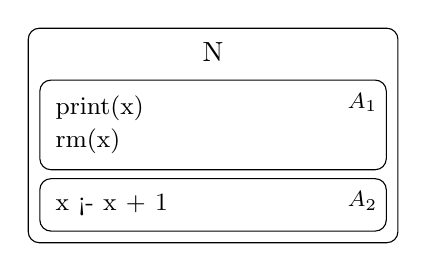
\begin{tikzpicture}
\node (0) {N};
\cell{c}{print(x)\\rm(x)}
\cell{a}{x <- x + 1}
\begin{pgfonlayer}{background}
    \draw[rounded corners] ($(current bounding box.south west) - (4pt, 4pt)$) rectangle ($(current bounding box.north east) + (4pt, 2pt)$);
\end{pgfonlayer}
\end{tikzpicture}
\gdef\SatexReachedEnd{}
\end{document}
